\documentclass[letter, 10pt]{article}
\usepackage[latin1]{inputenc}
\usepackage[spanish]{babel}
\usepackage{amsfonts}
\usepackage{amsmath}
\usepackage[dvips]{graphicx}
\usepackage{url}
\usepackage[top=3cm,bottom=3cm,left=3.5cm,right=3.5cm,footskip=1.5cm,headheight=1.5cm,headsep=.5cm,textheight=3cm]{geometry}

\usepackage{float}

\begin{document}
\title{Inteligencia Artificial \\ \begin{Large}Informe Final: 2D Strip Packing Problem\end{Large}}
\author{Florencia Ram\'irez Sancristoful}
\date{20 de noviembre de 2023}
\maketitle


%--------------------No borrar esta secci\'on--------------------------------%
\section*{Evaluaci\'on}

\begin{tabular}{ll}
C\'odigo Fuente (20\%): &  \underline{\hspace{2cm}}\\
Representaci\'on (15\%):  & \underline{\hspace{2cm}} \\
Descripci\'on del algoritmo (20\%):  & \underline{\hspace{2cm}} \\
Experimentos (10\%):  & \underline{\hspace{2cm}} \\
Resultados (10\%):  & \underline{\hspace{2cm}} \\
Conclusiones (20\%): &  \underline{\hspace{2cm}}\\
Bibliograf\'ia (5\%): & \underline{\hspace{2cm}}\\
 &  \\
\textbf{Nota Final (100)}:   & \underline{\hspace{2cm}}
\end{tabular}
%---------------------------------------------------------------------------%

% Esto supongo que lo comento despues
\vspace{0.6cm}


\begin{abstract}
    Resumen del informe en no m\'as de 10 l\'ineas, donde se sintetice el problema que se trata, el acercamiento propuesto y sirva para que un lector no involucrado comprenda el objetivo del documento.
    \vspace{0.2cm}    
    El \emph{2D Strip Packing Problem} es un problema de optimizaci\'on en el cual un conjunto de elementos deben ser posicionados en una regi\'on definida cumpliendo ciertas condiciones con el objetivo de minimizar el espacio necesario para ajustar estos elementos. Se han propuesto una gran variedad de m\'etodos y modelos para la resoluci\'on de este problema y variantes existentes, se presentan los m\'etodos m\'as relevantes y conocidos para luego realizar un an\'alisis comparativo entre ellos con un enfoque la variante con rotaciones y sin cortes en guillotina.

\end{abstract}

\section{Introducci\'on}

El \emph{2D Strip Packing Problem} (2DPP) es un problema de gran inter\'es estudiado por diversas industrias, derivado de los problemas de empaquetamiento y est\'a enfocado en la optimizaci\'on del espacio. Este problema consiste en ordenar, sin solapar, un conjunto de elementos rectangulares, cada uno con dimensiones conocidas, en una regi\'on de ancho fijo pero alto infinito, teniendo como objetivo final minimizar el \'area inutilizada de dicha regi\'on.

Este trabajo tiene por objetivo enfatizar la importancia del 2DSPP, presentando el estado del arte de este problema, dando a conocer las t\'ecnicas de resoluci\'on m\'as relevantes existentes en la literatura actual. Analizando las ventajas y desventajas que tienen, para compararlas entre s\'i, midiendo la eficiencia y calidad de las soluciones encontradas por cada uno de estos m\'etodos mencionados.

Dado que el 2DSPP tiene una gran cantidad de aplicaciones pr\'acticas reales en la actualidad~\cite{junior2022rectangular}~\cite{vasilyev2023generalized}, el desarrollo de este trabajo est\'a impulsado por el deseo de contribuir a futuras investigaciones en la b\'usqueda e innovaci\'on de nuevos m\'etodos de resoluci\'on, de modo que puedan adaptarse a los cambios del futuro y sigan brindando soluciones eficientes a este problema.

El resto de las secciones de este documento est\'an estructuradas de la siguiente manera, en la secci\'on 2 se explican los conceptos fundamentales del 2DSPP. En la secci\'on 3 se presenta el Estado del Arte del problema. En la secci\'on 4 se analizan algunos modelos matem\'aticos que entregan una soluci\'on al problema. En la secci\'on 5 se propone una representaci\'on para la resoluci\'on de este problema y en la secci\'on 6 se expone el algoritmo propuesto. En la secci\'on 7 se realizan pruebas para comparar el rendimiento de este algoritmo respecto a las soluciones entregadas por t\'ecnicas anteriores, que luego son presentadas y analizadas en la secci\'on 8. Finalmente, en la secci\'on 9 se presentan las conclusiones.

\section{Definici\'on del Problema}

El \emph{2D Strip Packing Problem} es un problema combinatorial de optimizaci\'on derivado de los problemas de empaquetamiento~\cite{oliveira2016survey}, en el cual se deben ajustar una serie de elementos rectangulares, con un ancho y alto definido, en una regi\'on rectangular de ancho y alto infinito, minimizando el \'area total inutilizada de la regi\'on o minimizando la altura total de la regi\'on. Este es un problema NP-Complejo conocido con bastantes aplicaciones en diversas industrias, incluyendo industrias madereras, vidrieras, metal\'urgicas, textiles, entre otras~\cite{lodi2002two}~\cite{vasilyev2023generalized}.

Al ser un problema NP-Complejo, ha sido estudiado de manera amplia con anterioridad y una de las limitaciones, o dificultades, que ha presentado es que los algoritmos de resoluci\'on propuestos en la literatura se dividen en tres tipos, los m\'etodos exactos, los m\'etodos heur\'isticos y los m\'etodos h\'ibridos~\cite{he2013heuristics}~\cite{junior2023framework}~\cite{oliveira2016survey}~\cite{wei2017improved}.

Los m\'etodos exactos resuelven este problema encontrando la soluci\'on \'optima, pero no pueden resolver instancias de mayor tama\~no eficientemente. Los m\'etodos heur\'esticos buscan una soluci\'on de buena calidad, pero no aseguran que la soluci\'on sea \'optima. Los m\'etodos h\'ibridos combinan diversos m\'etodos para encontrar una soluci\'on de buena calidad. Por lo que, hasta el momento no se han encontrado formas de obtener la soluci\'on \'optima y resolver este problema de manera eficiente en las situaciones reales m\'as complejas~\cite{thomas2013hybrid}.

\subsection{Variables, restricciones y objetivos}

Antes de definir las variables de este problema, es necesario identificar las constantes ya existentes. Las cuales corresponden a la cantidad de elementos rectangulares a posicionar, el ancho definido de la regi\'on y las dimensiones de cada elemento.

Una vez identificadas estas constantes, se pueden definir tres variables para la resoluc\'on de este problema. Dos variables correspondientes a la posici\'on que tomar\'a cada elemento, tomando como referencia un plano cartesiano, y una variable correspondiente al indicador de rotaci\'on de cada elemento. Adem\'as, estas variables se ven restringidas por las siguientes condiciones:

\begin{enumerate}
    \item Cada elemento debe estar posicionado dentro de los m\'argenes de la regi\'on.
    \item Los elementos no pueden solaparse, en otras palabras, dos elementos no pueden estar en la misma posici\'on.
\end{enumerate}

El objetivo de este problema es acomodar todos estos elementos minimizando la cantidad de espacio inutilizado en la regi\'on, esto puede ser logrado minimizando la altura de la regi\'on.

\subsection{Problemas relacionados y variantes m\'as conocidas}

El \emph{2D Strip Packing Problem} es considerado un subproblema de los llamados \emph{Packing Problems} (PP)~\cite{babaouglu2017solving}~\cite{lodi2002two}, tambi\'en conocidos como problemas de empaquetamiento en espa\~nol, en los cuales se deben acomodar objetos en contenedores espec\'ificos y tiene dos posibles objetivos, utilizar la menor cantidad de contenedores posibles o ajustar todos estos objetos en un \'unico contenedor desperdiciando la menor cantidad de espacio posible.

Algunas de las caracter\'isticas que pueden cambiar en las variantes de este problema son las dimensiones, tipos de cortes o patrones, conocimiento previo de los elementos, formas, ortogonalidad y rotaci\'on~\cite{junior2022rectangular}~\cite{oliveira2016survey}.

Entre estas posibles variantes, son normalmente conocidos cuatro subproblemas que consideran limitaciones relacionadas a la rotaci\'on y corte de los elementos~\cite{junior2022rectangular}~\cite{lodi2002two}. En relaci\'on a la rotaci\'on de estos elementos, tienen una orientaci\'on fija que no se puede modificar (O) o pueden ser rotados en 90\textdegree (R), y en relaci\'on al tipo de corte de estos, se deben acomodar para permitir cortes en guillotina (G) o pueden ser posicionados libremente (F). Considerando estas caracter\'isticas, se identifica la variante RF que tiene la menor cantidad de restricciones y, en consecuencia, es considerada como la m\'as f\'acil de resolver. Si se fija la orientaci\'on de estos elementos, no pueden ser rotados, se define la variante OF. Finalmente, si se imponen los cortes en guillotina se pueden identificar las versiones RG y OG, permitiendo la rotaci\'on de los elementos o fijando su orientaci\'on, respectivamente. El estudio hecho en este informe tiene un enfoque en la variante RF, considera la posible rotaci\'on de los objetos y estos pueden ser posionados libremente en la regi\'on.

Tambi\'en, se distinguen dos categor\'ias respecto al conocimiento previo sobre los elementos~\cite{oliveira2016survey}. La primera categor\'ia es conocida como \emph{online} y en esta no se tiene conocimiento sobre c\'omo son los siguientes elementos a posicionar, implica que una vez posicionado un elemento este ya no puede ser movido. En cambio, la segunda categor\'ia, \emph{offline}, es la m\'as com\'un en investigaciones y se distingue por tener conocimiento previo de todos los elementos a posicionar, lo cual hace posible definir una secuencia sobre c\'omo ser\'an colocados.

Dos de los problemas m\'as similares son el \emph{Rectangular Packing Problem} y el \emph{Bin Packing Problem}. En el primero se deben ordenar una serie de rect\'angulos en una regi\'on de ancho y largo fijo con el objetivo de maximizar el \'area de estos rect\'angulos ajustados~\cite{chen2007two}. Por otro lado, en el segundo se debe ajustar una serie de elementos en una cantidad finita de contenedores de ancho y alto fijo, tiene como objetivo minimizar la cantidad de contenedores utilizados~\cite{lodi2002two}.

\section{Estado del Arte}

El \emph{2D Strip Packing Problem} (2DSPP) es uno de los problemas de empaquetamiento m\'as simples que surge de la necesidad de reducir los costos operacionales de las industrias transformadoras de materias primas~\cite{junior2022rectangular}, por lo cual ha sido estudiado intensamente y se han propuesto diversos m\'etodos para su resoluci\'on, los cuales pueden ser divididos en tres categor\'ias, m\'etodos exactos, heur\'isticos e h\'ibridos.

Los m\'etodos exactos se caracterizan por encontrar la soluci\'on \'optima, los cuales funcionan cuando se tienen instancias m\'as peque\~nas a resolver ya que cuando intentan resolver instancias m\'as grandes los tiempos de ejecuci\'on son muy altos, como estos tiempos de ejecuci\'on son tan altos, no se considera como un m\'etodo eficiente. Los m\'etodos heur\'isticos no aseguran que la soluci\'on encontrada sea \'optima, tampoco reconocen la soluci\'on \'optima, pero se caracterizan por entregar una soluci\'on de buena calidad con tiempos de ejecuci\'on considerados bajos y, a diferencia de los m\'etodos exactos, los hace capaces de encontrar una soluci\'on cuando se tienen instancias de mayor tama\~no. Por \'ultimo, los m\'etodos h\'ibridos combinan aspectos de estos otros m\'etodos para entregar soluciones factibles a este problema.

La mayor\'ia de las investigaciones recientes se enfocan en los m\'etodos heur\'isticos e h\'ibridos, debido a que una de las principales limitaciones existentes es que no se ha logrado proponer un algoritmo de resoluci\'on que entregue la soluci\'on \'optima a este problema para instancias de mayor tama\~no. Las instancias de menor tama\~no son resueltas de manera eficiente por los m\'etodos ya existentes, por lo que no se considera necesario buscar algoritmos m\'as eficientes y se enfocan principalmente en buscar nuevas t\'ecnicas para la resoluci\'on de instancias m\'as grandes, que no pueden ser resueltas por los m\'etodos exactos.

\subsection{M\'etodos exactos}

Los m\'etodos exactos garantizan que la soluci\'on entregada es la \'optima y normalmente est\'an basados en modelos matem\'aticos~\cite{oliveira2016survey}. En comparaci\'on a todos las investigaciones hechas sobre los otros dos m\'etodos, existen menos investigaciones sobre los m\'etodos exactos y, debido a las restricciones computacionales de tiempos de ejecuci\'on y memoria, no son capaces de resolver instancias de gran tama\~no eficientemente~\cite{he2013heuristics}, lo que contribuye a la cantidad limitada de informaci\'on reciente y actualizada sobre estos m\'etodos.

La mayor\'ia de estos m\'etodos se basan en la estrategia \emph{Branch and Bound}, una forma de \emph{backtracking} que genera un \'arbol con todas las posibles soluciones y corta las ramas que dejan de ser \'optimas. Bas\'andose en una adaptaci\'on para el \emph{Contiguous Bin Packing Problem} (CBP) y modelos matem\'aticos propuestos~\cite{martello2003exact}, surgen los algoritmos \emph{STAIRCASE} y \emph{G-STAIRCASE}~\cite{kenmochi2009exact} que utilizan esta metodolog\'ia.

El primero obtiene un l\'imite inferior correspondiente a una altura $H$ propuesta, luego agrega elementos con dimensiones $1 \cdot 1$ hasta obtener una instancia de \emph{Perfect Packing} (PP), casos perfectos en los que no existen \'areas desperdiciadas, luego revisa si la instancia generada puede ser resuelta con una estrategia de posicionamiento en escalera considerando instancias PP. Si encuentra una soluci\'on v\'alida, termina la ejecuci\'on y $H$ corresponde a la soluci\'on \'optima, en caso contrario, incrementa en valor de $H$ en uno y repite este proceso. El segundo algoritmo tambi\'en obtiene un l\'imite inferior correspondiente a la altura $H$, pero no agrega elementos extra, luego revisa si puede ser resuelto utilizando la misma estrategia, este caso permite los espacios vac\'ios para generar en la regi\'on bajo la escalera y, al igual que el anterior, si encuentra una soluci\'on v\'alida termina, sino aumenta $H$ en uno.

Ambos algoritmos logran resolver la mayor\'ia de las instancias de prueba con un m\'aximo de 200 rec\'angulos en menos de una hora, y concluyen que estos algoritmos son una alternativa a los propuestos anteriormente, considerando que la mayor\'ia de los algoritmos existentes hasta ese momentos estaban enfocados en la variante OF.

\subsection{M\'etodos heur\'isticos}

Estos m\'etodos son una alternativa a los m\'etodos exactos, dado que los \'ultimos no son capaces de entregar una soluci\'on de manera eficiente, los m\'etodos heur\'isticos, tambi\'en conocidos como m\'etodos aproximados, son capaces de brindar soluciones de buena calidad en bajos tiempos. A diferencia de los m\'etodos exactos, no buscan la soluci\'on \'optima y, si la encuentran, no son capaces de reconocerla.

La primera heur\'istica propuesta en la literatura fue \emph{Bottom Left} (BL)~\cite{oliveira2016survey} y es una de las estrategias m\'as reconocidas, pertenece al conjunto de estrategias que selecciona un elemento y despu\'es identifica el espacio disponible m\'as apto para posicionarlo. El objetivo de BL es posicionar cada elemento lo m\'as abajo y a la izquierda posible y tiene la ventaja de ser considerado eficiente y simple, pero una de sus mayores desventajas es su incapacidad de rellenar los espacios vac\'ios rodeados de elementos ya posicionados. En base a esta metodolog\'ia surgen \emph{Bottom Left Fill} (BLF), una variante que considera estos espacios que eran desperdiciados, e \emph{Improved Bottom Left} (iBL), una variante mejorada de BL que le da prioridad a los movimientos hacia abajo y los mueve a la izquierda lo suficiente para que sigan bajando. 

Tambi\'en existen las estrategias que est\'an enfocadas en asignar el mejor elemento a un espacio libre determinado y su primera heur\'istica propuesta fue \emph{Best Fit} (BF)~\cite{verstichel2013improved}. Esta selecciona un espacio libre lo m\'as abajo posible y luego busca un elemento que quepa perfectamente, si no existe este elemento se escoge el elemento m\'as grande que quepa en dicho espacio y tiene tres posibles posiciones, lo m\'as a la izquierda posible, junto al elemento de mayor altura o junto al elemento de menor altura. Con el m\'etodo BF surgi\'o el concepto de \emph{skyline}, por lo que se proponen m\'etodos mejorados que pueden resolver eficientemente instancias de tama\~no grande, \emph{Three-way Best Fit} (TwBF) que agrega tres nuevos criterios para posicionar los elementos, y \emph{Fast Layer-Based Heuristic} (FH) que propone mantener la l\'inea del \emph{skyline} lo m\'as plana posible utilizando una llamada \emph{fitness function}. Esta funci\'on utiliza una escala de 4 valores para determinar qu\'e elemento es el m\'as apto para asignarlo a un espacio libre espec\'ifico, siendo 0 el peor y 4 el mejor. Utilizando esta \emph{fitness function} y la idea de mantener el \emph{skyline} lo m\'as plano posible se proponen diversas mejoras como \emph{Intelligent Search Algorithm} (ISA) y \emph{Hybrid Demon Algorithm} (HDA), ambos usando una escala con cinco posibles valores, \emph{Simple Randomized Algorithm} (SRA) y \emph{Efficient Intelligent Search Algorithm} (IA)~\cite{wei2016efficient}, los cuales ocupan una escala de ocho valores.

Otros m\'etodos que no entran en estas dos categor\'ias son \emph{Heuristic Recursive Algorithm} (HR) y \emph{Deterministic Heuristic Algorithm} (DHA)~\cite{he2013heuristics}. El primero utiliza la t\'ecnica dividir y conquistar y en cada iteraci\'on divide el espacio vac\'io en dos subespacios, soluciona recursivamente cada uno y finalmente combina las soluciones, su principal desventaja es el orden en que se posicionan los elementos afecta la eficiencia de este algoritmo. El segundo se compone de dos fases, la primera fase utiliza una estrategia \emph{greedy} para posicionar los elementos y la segunda fase aplica una b\'usqueda parcial utilizando \'arboles para encontrar la posici\'on que minimice la altura. 

\subsection{M\'etodos h\'ibridos}

Los m\'etodos h\'ibridos, como su nombre lo indica, brindan soluciones de buena calidad de manera eficiente combinando el uso de diversos algoritmos. Surgen bajo la idea de obtener una soluci\'on inicial que luego va a ser mejorada usando otro algoritmo. Es com\'un el uso de \emph{Genetic Algorithm} (GA), \emph{Simulated Annealing} (SA) o \emph{Tabu Search} (TS) para generar la soluci\'on inicial y son normalmente usados con los algoritmos BL, BF y todas sus versiones mejoradas.

GA utiliza una analog\'ia de la selecci\'on natural, a todas las posibles soluciones de un problema se le asigna un valor bas\'andose en una \emph{fitness function}~\cite{thomas2013hybrid}, lo que finalmente se utiliza para generar una secuencia de los elementos a posicionar. SA surge como una variante del m\'etodo \emph{Hill-Climbing} (HC)~\cite{hopper2001empirical}, una t\'ecnica de b\'usqueda local que se mueve entre las soluciones de un vecindario, si se encuentra una mejor soluci\'on realiza el cambio y sigue con la b\'usqueda hasta no encontrar mejoras dentro del vecindario. SA soluciona este problema aceptando soluciones de peor calidad en base a una probabilidad asociada a la diferencia de la calidad de esta soluci\'o. TS, al igual que SA, es una t\'ecnica de b\'usqueda local derivada de HC~\cite{wei2011skyline}, a la cual se le adjunta una memoria a corto plazo, para guardar las \'ultimas soluciones y evitar los ciclos entre las mismas.

\subsection{Comparaciones entre m\'etodos}

Los resultados computacionales de los m\'etodos exactos \emph{STAIRCASE} y \emph{G-STAIRCASE}~\cite{kenmochi2009exact} en el cuadro~\ref{tab:comparacion_beng10} muestran que ambos algoritmos pueden resolver instancias de hasta 200 elementos, y la soluci\'on \'optima entregada es igual, o muy cercana, al l\'imite inferior calculado, pero entre ambos algoritmos \emph{STAIRCASE} obtiene mejores resultados agregando los elementos indicados por la columna $1 \cdot 1$, destancando los menores tiempos de ejecuci\'on.

\renewcommand{\arraystretch}{1.1}
\begin{table}[H]
    \centering
    \begin{tabular}{|l|lllll|rr|}
    \hline
    Instancia & \multicolumn{1}{l}{$N$} & \multicolumn{1}{l}{$W$} & \multicolumn{1}{l}{$LW$} & \multicolumn{1}{l}{$H$} & \multicolumn{1}{l|}{$1 \cdot 1$} & \multicolumn{1}{l}{\emph{STAIRCASE}} & \multicolumn{1}{l|}{\emph{G-STAIRCASE}} \\ \hline
    beng01 & 20 & 25 & 30 & 30 & 9 & \textbf{0.08} & \textbf{0.08} \\ \hline
    beng02 & 40 & 25 & 57 & 57 & 5 & 0.12 & \textbf{0.10} \\ \hline
    beng03 & 60 & 25 & 84 & 84 & 10 & \textbf{0.10} & \textbf{0.10} \\ \hline
    beng04 & 80 & 25 & 107 & 107 & 2 & \textbf{0.08} & 0.13 \\ \hline
    beng05 & 100 & 25 & 134 & 134 & 20 & \textbf{0.08} & 0.13 \\ \hline
    beng06 & 40 & 40 & 36 & 36 & 20 & \textbf{0.10} & 0.12 \\ \hline
    beng07 & 80 & 40 & 67 & 67 & 7 & \textbf{0.11} & \textbf{0.11} \\ \hline
    beng08 & 120 & 40 & 101 & 101 & 13 & \textbf{0.17} & 0.18 \\ \hline
    beng09 & 160 & 40 & 126 & 126 & 32 & \textbf{0.23} & 0.41 \\ \hline
    beng10 & 200 & 40 & 156 & 156 & 23 & \textbf{0.81} & 3.53 \\ \hline
    \end{tabular}
    \caption{Tiempo de ejecuci\'on [s] de los algoritmos para entregar la soluci\'on \'optima.}
    \label{tab:comparacion_beng10}
\end{table}

Las comparaciones~\cite{hopper2001empirical} entre los m\'etodos h\'ibridos y heur\'isticos destacan los m\'etodos que obtuvieron la menor diferencia relativa entre la soluci\'on entregada y la soluci\'on \'optima. Considerando todas las instancias presentadas en el cuadro~\ref{tab:comparacion_c7} y sus resultados respectivos se concluye que el m\'etodo h\'ibrido SA + BLF obtuvo el mejor rendimiento, mientras que el m\'etodo heur\'istico BL obtuvo las mayores diferencias. Estos resultados son acorde a lo presentado en la literatura, el algoritmo BL fue uno de los primeros propuestos, BLF es una versi\'on mejorada de este y mejora la soluci\'on entregada con SA.

\begin{table}[H]
    \centering
    \begin{tabular}{|l|rrrrrrr|}
    \hline
    M\'etodo & \multicolumn{1}{l}{C1} & \multicolumn{1}{l}{C2} & \multicolumn{1}{l}{C3} & \multicolumn{1}{l}{C4} & \multicolumn{1}{l}{C5} & \multicolumn{1}{l}{C6} & \multicolumn{1}{l|}{C7} \\ \hline
    GA + BL & 6 & 10 & 8 & 9 & 11 & 15 & 21 \\ \hline
    SA + BL & \textbf{4} & 7 & 7 & 6 & 6 & 7 & 13 \\ \hline
    HC + BL & 9 & 18 & 11 & 14 & 14 & 20 & 25 \\ \hline
    BL & 17 & 31 & 24 & 18 & 18 & 21 & 29 \\ \hline
    GA + BLF & \textbf{4} & 7 & \textbf{5} & \textbf{3} & 4 & 4 & 5 \\ \hline
    SA + BLF & \textbf{4} & \textbf{6} & \textbf{5} & \textbf{3} & \textbf{3} & \textbf{3} & \textbf{4} \\ \hline
    HC + BLF & 7 & 10 & 7 & 7 & 6 & 7 & 7 \\ \hline
    BLF & 11 & 16 & 12 & 5 & 5 & 5 & 5 \\ \hline
    \end{tabular}
    \caption{Distancia relativa (\%) entre la soluci\'on entregada y la soluci\'on \'optima.}
    \label{tab:comparacion_c7}
\end{table}

Al comparar el algoritmo DHA~\cite{he2013heuristics} con otros m\'etodos h\'ibridos y heur\'isticos previos se destaca en el cuadro~\ref{tab:comparacion_c21} las soluciones \'optimas encontradas y se puede observar c\'omo este algoritmo nuevo supera a los dem\'as y en los casos donde no encuentra la soluci\'on \'optima est\'a muy cercana a ella, mientras que en las instancias de mayor tama\~no y complejidad es capaz de obtener esta soluci\'on \'optima en la mitad de estas.

\begin{table}[H]
    \centering
    \begin{tabular}{|l|lll|rrrrr|}
    \hline
    Instancia & $N$ & $W$ & $H_{opt}$ & \multicolumn{1}{l}{BF + TS} & \multicolumn{1}{l}{BF + SA} & \multicolumn{1}{l}{BF + GA} & \multicolumn{1}{l}{FH} & \multicolumn{1}{l|}{DHA} \\ \hline
    C11 & 16 & 20 & 20 & \textbf{20} & \textbf{20} & \textbf{20} & \textbf{20} & \textbf{20} \\ \hline
    C23 & 25 & 40 & 15 & 16 & 16 & 16 & \textbf{15} & \textbf{15} \\ \hline
    C33 & 28 & 60 & 30 & 31 & 31 & 31 & 32 & \textbf{30} \\ \hline
    C42 & 49 & 60 & 60 & 62 & 61 & 62 & 61 & 61 \\ \hline
    C51 & 73 & 60 & 90 & 92 & 91 & 92 & 91 & \textbf{90} \\ \hline
    C63 & 97 & 80 & 120 & 122 & 122 & 122 & 121 & \textbf{120} \\ \hline
    C71 & 196 & 120 & 240 & 245 & 244 & 245 & 241 & 241 \\ \hline
    \end{tabular}
    \caption{Soluciones entregadas por los m\'etodos BF+TS, BF+SA, BF+GA, FH y DHA.}
    \label{tab:comparacion_c21}
\end{table}

\section{Modelo Matem\'atico}

Los modelos presentados en la literatura~\cite{he2013heuristics}~\cite{hopper2001empirical}~\cite{kenmochi2009exact}~\cite{oliveira2016survey} para la resoluci\'on de las diversas variantes del 2DSPP tienen en com\'un algunos de los aspectos b\'asicos m\'as relevantes de este problema, por lo cual, en base a estos modelos se combinan y propone el siguiente modelo matem\'atico para la resoluci\'on de la variante RF, que permite rotaciones y posiciones libres.

\subsection{Constantes}

La definici\'on de este problema define tres constantes, las cuales representan el conocimiento previo de este problema y aportan a su resoluci\'on. La primera constante corresponde al ancho fijo de la regi\'on y, debido a la definici\'on de medida, este valor debe ser un n\'umero entero mayor que 0.
\begin{flalign*}
    & W = \text{ancho predefinido de la regi\'on}\ &
\end{flalign*}

La segunda constante corresponde a la cantidad total de elementos rectangulares que se deben ajustar en dicha regi\'on de ancho $W$, este valor tambi\'en debe ser un n\'umero entero mayor que 0, al igual que el ancho, por la definici\'on de cantidad, y la \'ultima constante corresponde a las dimensiones de cada uno de estos $N$ elementos rectangulares, estas dimensiones est\'an representadas de la forma $ancho \cdot alto$.
 \begin{flalign*}
    & N = \text{cantidad de elementos rectangulares}\ & \\
    & w_{i} \cdot h_{i} = \text{dimensiones del elemento}\ i, \hspace{0.1cm} \forall i \in [1,N]\ &
\end{flalign*}

\subsection{Variables}

Considerando que se representa la variante RF, permitiendo rotaciones y posiciones libres, se definen tres variables de decisi\'on. Dos de estas corresponden a la posici\'on de la esquina inferior izquierda de los elementos, tomando un plano cartesiano como referencia, estas posiciones ser\'an de la forma ($x_{i}$, $y_{i}$).
\begin{flalign*}
    & (x_{i}, y_{i}) = \text{posici\'on de la esquina inferior izquierda del elemento}\ i, \hspace{0.1cm} \forall i \in [1,N] &
\end{flalign*}

La \'ultima variable de decisi\'on corresponde una variable binaria representando el \'indice de rotaci\'on de los elementos, indicando con los valores 1 y 0, si se rota o no dicho elemento, respectivamente.
\begin{flalign*}
    & r_{i} =
    \begin{cases}
      1, & \text{se rota el elemento}\ i, \hspace{0.1cm} \forall i \in [1,N]\\
      0, & \text{caso contrario}
    \end{cases} &
\end{flalign*}

\subsection{Objetivos}

Su objetivo principal es minimizar el \'area $A$ sin utilizar de la regi\'on, lo cual puede ser logrado minimizando la altura $H$ de dicha regi\'on.
\begin{flalign*}
    & \min H = \min \{ \max_{i \in [1,N]} \{ y_{i} + h{_i} + r_{i} \cdot (w_{i} - h_{i}) \} \} &
\end{flalign*}

\subsection{Restricciones}

Esta variante define algunas condiciones que deben cumplir estas variables de decisi\'on, por lo que se identifican tres restricciones en total, dos de estas son parte de la definici\'on del problema y una de estas resulta de las variables de decisi\'on.

\vspace{0.2cm}
\textbf{Restricci\'on 1:} Los elementos no pueden superar el ancho $W$ de la regi\'on.
\begin{align}
    & x_{i} + w_{i} + r_{i} \cdot (h_{i} - w_{i}) \leq W, \hspace{0.1cm} \forall i \in [1,N] &
\end{align}

La restricci\'on considera la posible rotaci\'on del elemento $i$, si el \'indice de rotaci\'on es 0, el elemento $i$ utiliza el espacio entre los puntos $x_{i}$ y $x_{i} + w_{i}$ en el eje $x$ del plano cartesiano. En cambio, si el \'indice es 1, significando que el elemento $i$ es rotado en 90\textdegree, utilizar\'a el espacio entre los puntos $x_{i}$ y $x_{i} + h_{i}$.

\vspace{0.2cm}
\textbf{Restricci\'on 2:} Los elementos no pueden solaparse entre s\'i.
\begin{align}
    & x_{i} + w_{i} + r_{i} \cdot (h_{i} - w_{i}) \leq x_{j} \vee x_{j} + w_{j} + r_{j} \cdot (h_{j} - w_{j}) \leq x_{i} \vee & \\ \nonumber
    & y_{i} + h_{i} + r_{i} \cdot (w_{i} - h_{i}) \leq y_{j} \vee y_{j} + h_{j} + r_{j} \cdot (w_{j} - h_{ij}) \leq y_{i},\hspace{0.1cm} \forall i,j \in [1,N], i \neq j &
\end{align}

Esta restricci\'on aplica el mismo principio que la restricci\'on anterior. Si se tienen dos elementos $i, j$ existen cuatro posibles casos. El elemento $i$ puede estar a la izquierda, derecha, debajo o sobre el elemento $j$. Mientras se cumpla al menos uno de los posibles casos, debido al operador l\'ogico $\vee$, significa que los elementos no se solapan.

\vspace{0.2cm}
\textbf{Restricci\'on 3:} Naturaleza de las variables.
\begin{align}
    & x_{i}, y_{i} \geq 0, \hspace{0.1cm} x_{i}, y_{i} \in \mathbb{Z}, \hspace{0.1cm} r_{i} \in \{0,1\}, \hspace{0.1cm} \forall i \in [1,N] &
\end{align}

Usando un plano cartesiano como referencia, se considera que el ancho de la regi\'on va desde el punto (0, 0) al punto ($W$, 0) y si alguna de las variables de posici\'on de los elementos tiene un valor negativo, significa que fue colocado fuera de los m\'argenes establecidos de la regi\'on. Por la definici\'on de las constantes, las dimensiones de los elementos corresponden a un n\'umero entero, no considera decimales. Por \'ultimo, las variables del \'indice de rotaci\'on de los objetos corresponde a una variable binaria, lo que significa que sus \'unicos valores posibles son 0 o 1.

\section{Representaci\'on}

Para la resoluci\'on de este problema se seguir\'a la l\'ogica de la heur\'istica BL para el posicionamiento de los rect\'angulos, con el objetivo final de minimizar el \'area inutilizada, lo cual se hace minimizando la altura. Se presentan 4 representaciones en total, una se utiliza para representar los rect\'angulos, una para la posici\'on y rotaci\'on de estos rect\'angulos, una para el orden en que ser\'an posicionados y una para la regi\'on en la que se colocan estos rect\'angulos, en la cual se va construyendo la soluci\'on final.

\subsection{Rect\'angulos}
Los rect\'angulos se representar\'an mediante una estructura llamada \emph{Rectangle}, la cual tiene los siguientes atributos:
\begin{itemize}
    \item Id del rect\'angulo.
    \item Ancho del rect\'angulo.
    \item Alto del rect\'angulo.
    \item Estructura \emph{Position}, la cual indica la posici\'on y rotaci\'on que tomaa el rect\'angulo en la soluci\'on. 
\end{itemize}

\subsection{Posiciones}

Las posiciones $(x,y)$ e \'indices de rotaci\'on de estos rect\'angulos se representar\'an mediante una estructura llamada \emph{Position}, la cual tiene los siguientes atributos:
\begin{itemize}
    \item Coordenada $x$ de la esquina inferior izquierda del rect\'angulo.
    \item Coordenada $y$ de la esquina inferior izquierda del rect\'angulo.
    \item \'Indice de rotaci\'on del rect\'angulo, lo que indica si es rotado o no.
\end{itemize}

\subsection{Orden}

Se utilizar\'a un vector de estructuras \emph{Rectangle} de tama\~no $n$, correspondiente a la cantidad de rect\'angulos, para representar el orden en que van a ser colocados estos rect\'angulos, estando en la posici\'on $i$ el $i$-\'esimo rect\'angulo que se agrega a la regi\'on.

La figura~\ref{fig:orden} ilustra el orden en que ser\'ian agregados 5 rect\'angulos a la regi\'on, en este ejemplo, el primer rect\'angulo que se posiciona es el rect\'angulo $R_4$, refiri\'endose al rect\'angulo con $id = 4$, mientras que el rect\'angulo $R_1$ va a ser el quinto y \'ultimo en ser posicionado.

\begin{figure}[H]
    \centering
    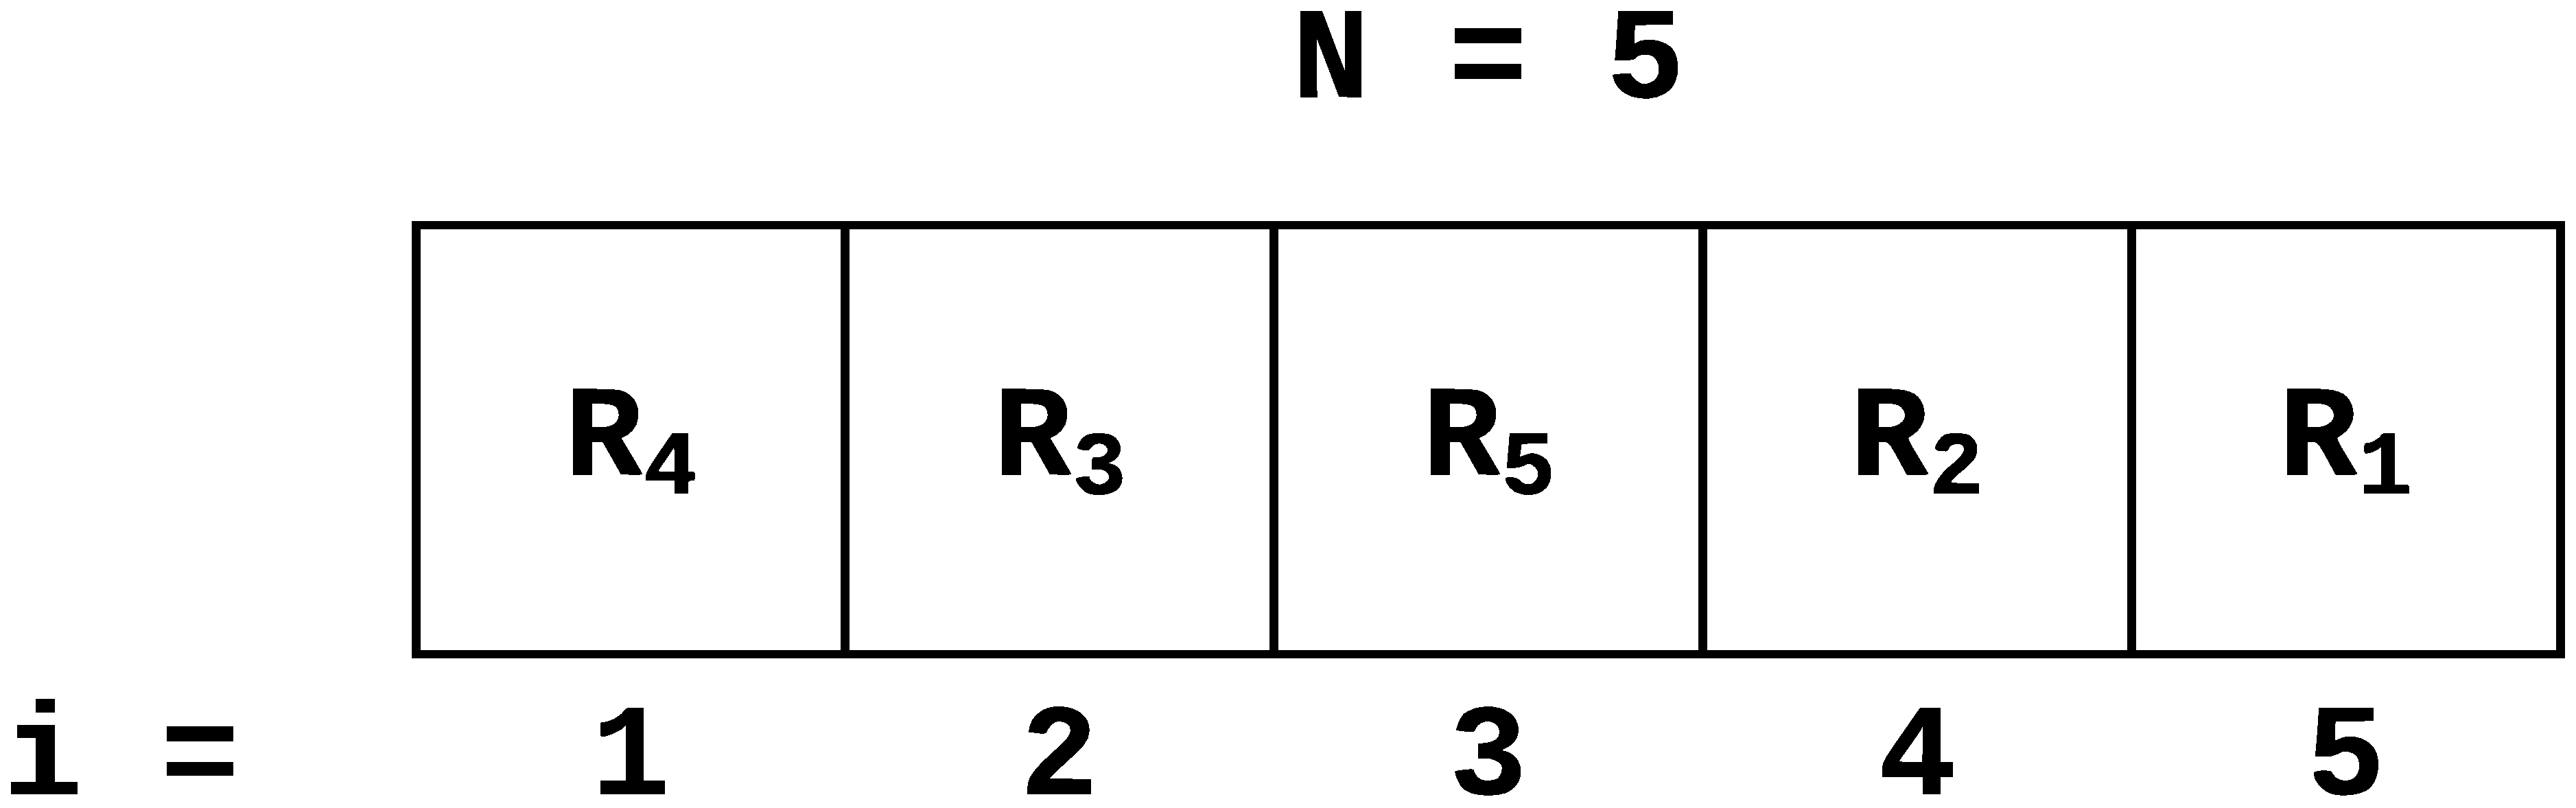
\includegraphics[width=0.45\textwidth]{images/orden.eps}
    \caption{Ejemplo de un vector de tama\~no 5.}
    \label{fig:orden}
\end{figure}

\subsection{Regi\'on}

La regi\'on de ancho fijo y alto infinito, en la cual se deben posicionar los rect\'angulos, se representar\'a con una clase llamada \emph{Strip}, la cual tiene los siguientes atributos:
\begin{itemize}
    \item Ancho fijo de la regi\'on.
    \item Vector de estructuras \emph{Rectangle}, indicando los rect\'angulos que ya fueron posicionados en la regi\'on.
\end{itemize}

La figura~\ref{fig:region} muestra las coordenadas e \'indices de rotaci\'on que toman 3 rect\'angulos una vez que son posicionados en la regi\'on, considerando que se agregan en el orden mencionado anteriormente.

\begin{figure}[H]
    \centering
    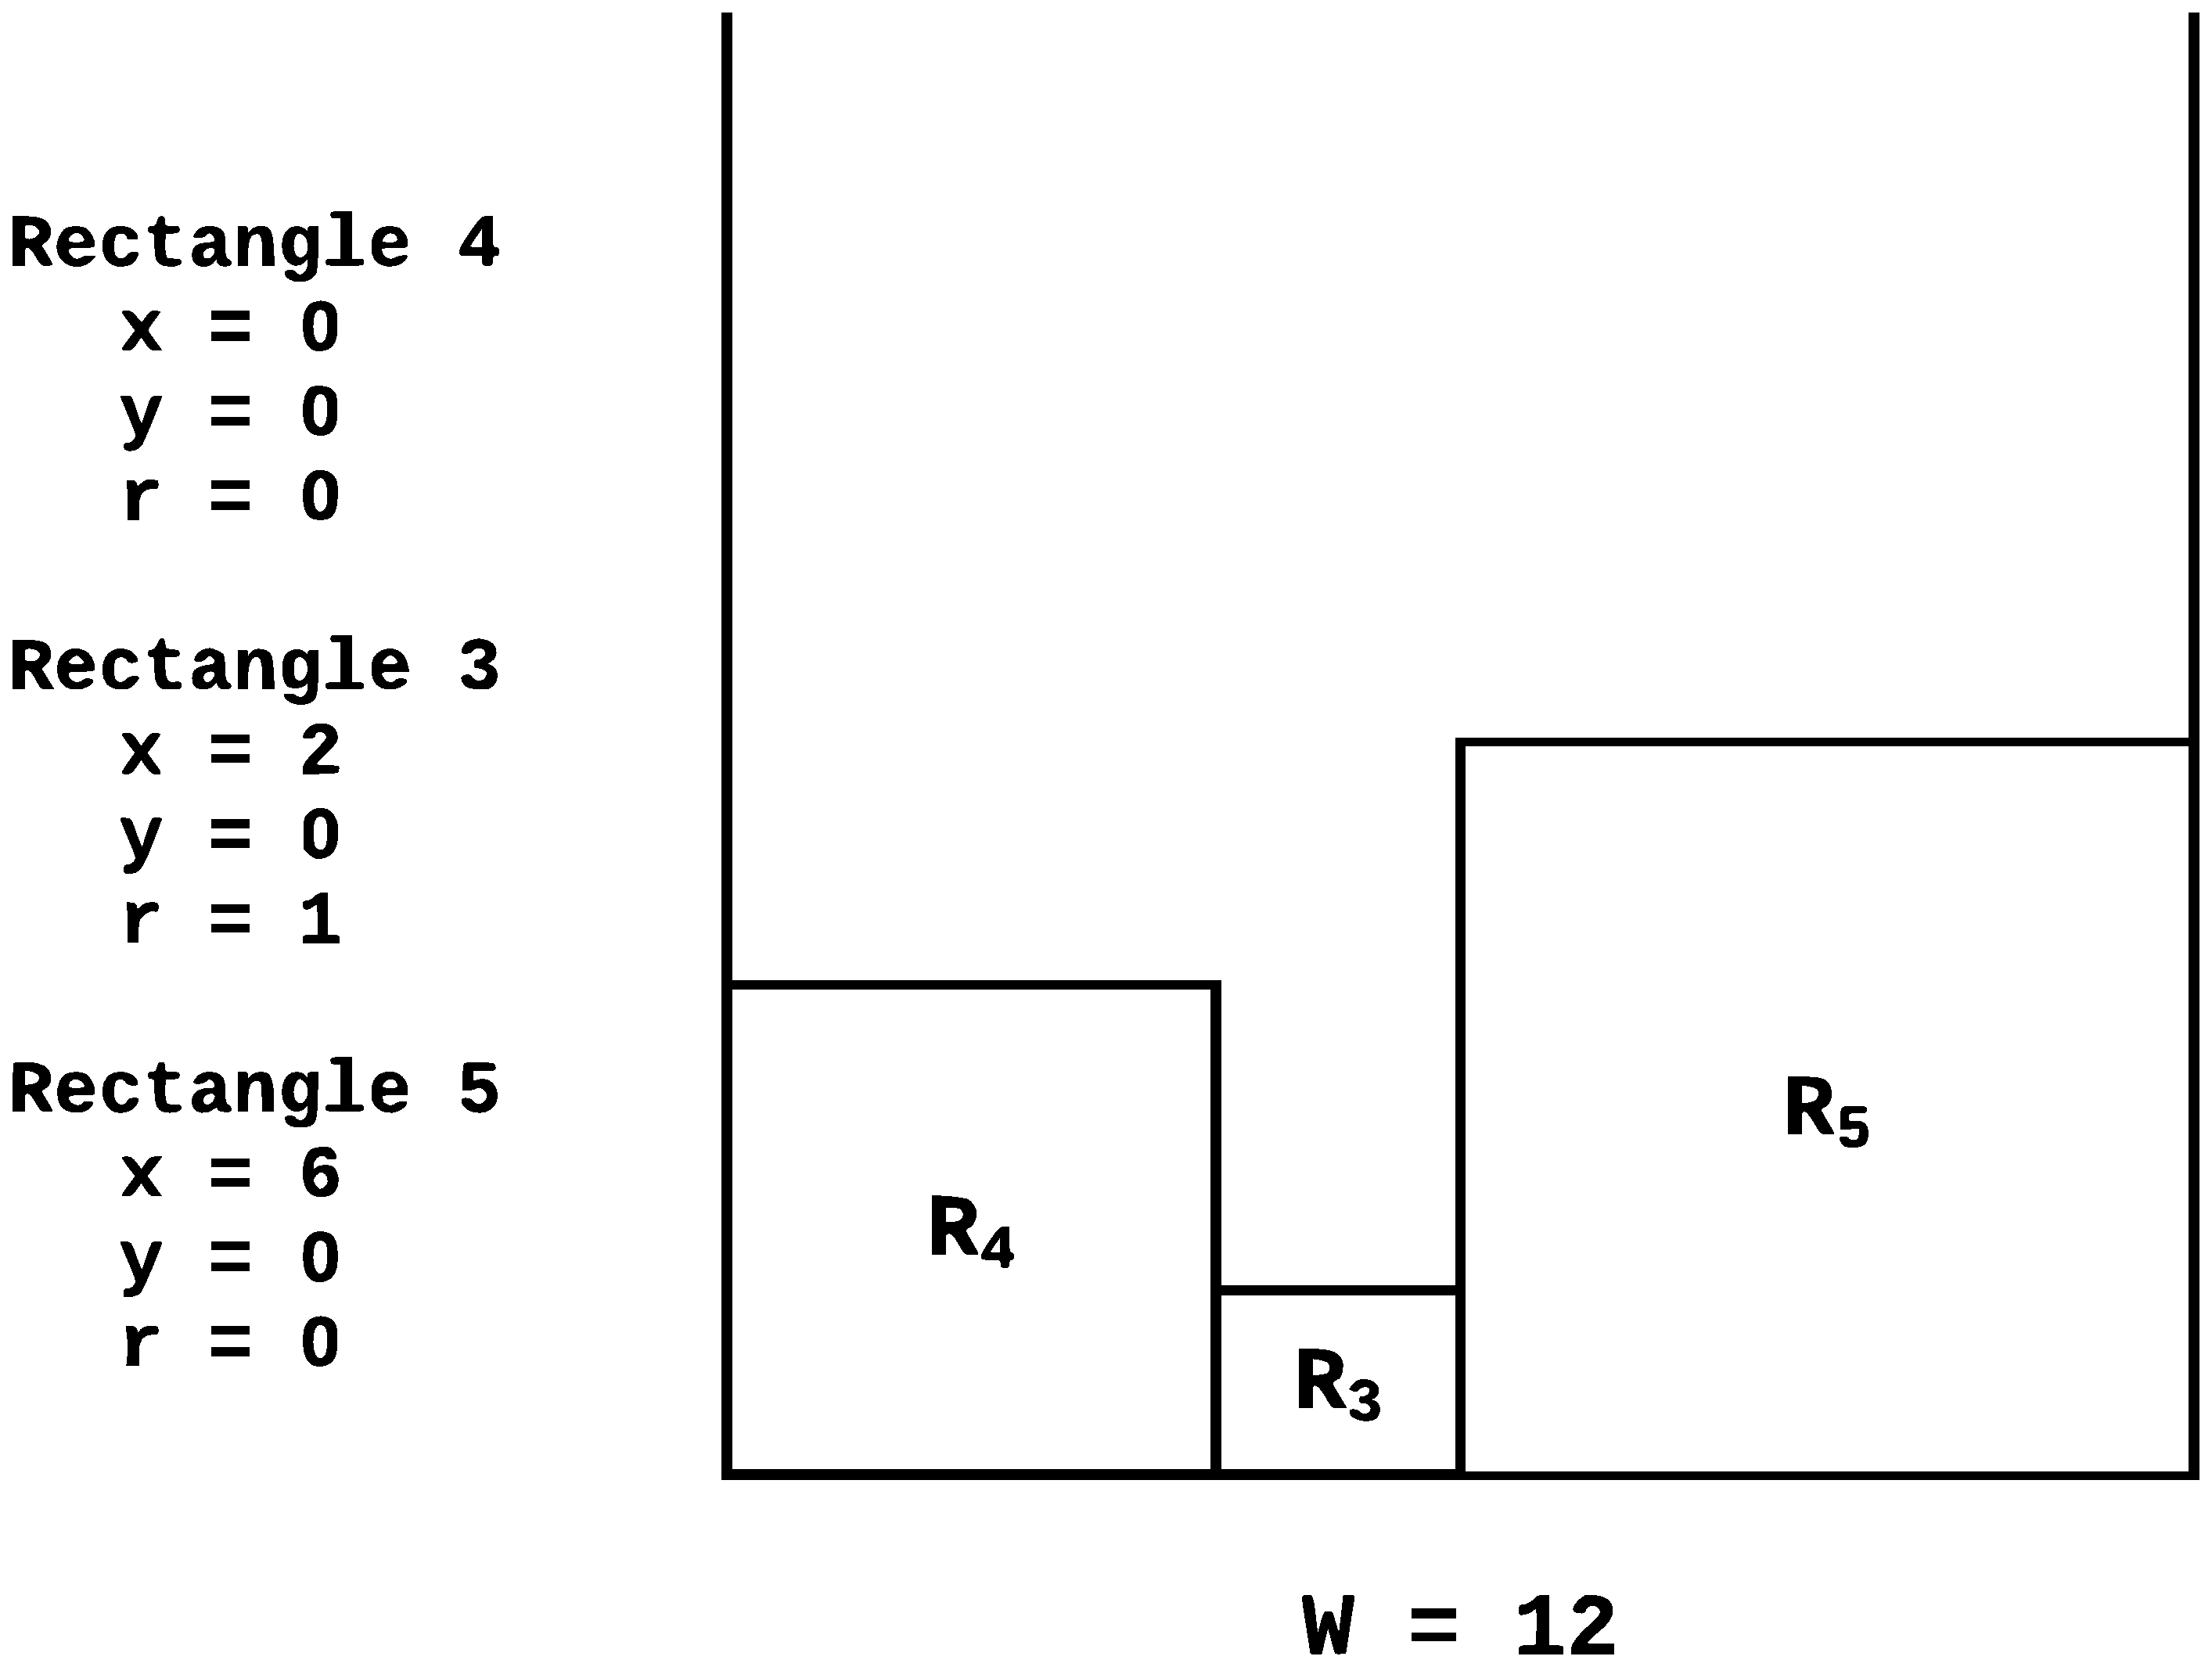
\includegraphics[width = 0.4\textwidth]{images/region.eps}
    \caption{Ejemplo del posicionamiento de 3 rect\'angulos siguiendo el orden mencionado.}
    \label{fig:region}
\end{figure}

\section{Descripci\'on del Algoritmo}

C\'omo fue implementada la soluci\'on. Interesa la implementaci\'on particular m\'as que el algoritmo gen\'erico, es decir, si se tiene que implementar SA, lo que se espera es que se explique en pseudoc\'odigo la estructura general y en p\'arrafos explicativos c\'omo fue implementada cada parte para su problema particular. Si se utilizan operadores/movimientos se debe justificar por qu\'e se utilizaron dichos operadores/movimientos. En caso de una t\'ecnica completa, describir detalles relevantes del proceso, si se utiliza recursi\'on o no, explicar c\'omo se van construyendo soluciones, cu\'ando se revisan restricciones, c\'omo se registran conflictos, etc. En este punto no se espera que se incluya c\'odigo, eso va aparte.

\section{Experimentos}

Se necesita saber c\'omo experimentaron, c\'omo definieron par\'ametros, 
c\'omo los fueron modificando, cu\'ales problemas/instancias se estudiaron y por qu\'e, etc. Recuerde que las t\'ecnicas completas son deterministas y las t\'ecnicas incompletas son estoc\'asticas.

\section{Resultados}

Qu\'e fue lo que se logr\'o con la experimentaci\'on, incluir tablas y gr\'aficos (lo m\'as explicativos posible). Los resultados deben ser comentados y justificados en detalle en esta secci\'on.

\section{Conclusiones}

Conclusiones RELEVANTES del estudio realizado. Incluir conclusiones acerca de la adecuaci\'on de la propuesta de soluci\'on al problema que se busca resolver. Listar y analizar ventajas y desventajas de la propuesta en base a los resultados obtenidos y comportamiento de la propuesta en diferentes escenarios (problemas/instancias/par\'ametros). Incluir trabajo futuro en base a las conclusiones.
\vspace{0.2cm}

El \emph{2D Strip Packing Problem} es un problema con diversas aplicaciones pr\'acticas reales, por lo cual es importante buscar soluciones buenas y eficientes para instancias de mayor tama\~no y complejidad, ya que estas son las que m\'as se asemejan a sus aplicaciones reales. Existen diversas t\'ecnicas enfocadas en las distintas variantes que existen, las restricciones que debe cumplir cada uno de estos m\'etodos depende de la variante de estudio, considerando algunas m\'as sencillas que otras. Los m\'etodos heur\'isticos e h\'ibridos son los m\'as favorables, dado que logran resolver las instancias m\'as parecidas a la realidad, pero a\'un no pueden obtener la soluci\'on \'optima para estas instancias m\'as complejas. Las investigaciones recientes respecto al problema est\'an enfocadas en estos m\'etodos y uno de los posibles trabajos a realizar en un futuro es crear nuevos m\'etodos h\'ibridos con las nuevas t\'ecnicas heur\'isticas m\'as competitivas hasta la fecha. 

\bibliographystyle{plain}
\bibliography{Referencias}

\end{document} 


